\documentclass{article} 
\usepackage{polski} %moze wymagac dokonfigurowania latexa, ale jest lepszy ni� standardowy babel'owy [polish] 
\usepackage[utf8]{inputenc}
\usepackage[OT4]{fontenc} 
\usepackage{graphicx,color} %include pdf's (and png's for raster graphics... avoid raster graphics!) 
\usepackage{url} 

% Zmiana rozmiar�w strony tekstu
\addtolength{\voffset}{-1cm}
\addtolength{\hoffset}{-1cm}
\addtolength{\textwidth}{2cm}
\addtolength{\textheight}{2cm}

%bardziej zyciowe parametry sterujace rozmieszczeniem rysunkow
\renewcommand{\topfraction}{.85}
\renewcommand{\bottomfraction}{.7}
\renewcommand{\textfraction}{.15}
\renewcommand{\floatpagefraction}{.66}
\renewcommand{\dbltopfraction}{.66}
\renewcommand{\dblfloatpagefraction}{.66}
\setcounter{topnumber}{9}
\setcounter{bottomnumber}{9}
\setcounter{totalnumber}{20}
\setcounter{dbltopnumber}{9}

% w�asny bullet list z malymi odstepami
\newenvironment{tightlist}{
\begin{itemize}
  \setlength{\itemsep}{1pt}
  \setlength{\parskip}{0pt}
  \setlength{\parsep}{0pt}}
{\end{itemize}}




%\title{Sprawozdanie z laboratorium:\\Metaheurystyki i Obliczenia Inspirowane Biologicznie}
%\author{}
%\date{}


\begin{document}

\thispagestyle{empty} %bez numeru strony

\begin{center}
{\large{Sprawozdanie z laboratorium:\\
Metaheurystyki i Obliczenia Inspirowane Biologicznie}}

\vspace{3ex}

Część I: Algorytmy optymalizacji lokalnej, problem ATSP
%Cz��� II: Algorytmy optymalizacji lokalnej i globalnej, problem QAP
%Cz��� III: Eksperyment: ... (prezentacj� mo�na zrobi� w LaTeX/klasa beamer)

\vspace{3ex}
{\footnotesize\today}

\end{center}


\vspace{10ex}

Prowadzący: dr inż. Maciej Komosiński

\vspace{5ex}

Autorzy:
\begin{tabular}{lllr}
\textbf{Konrad Olczak} & inf80061 & SKiSR & kolczak87@gmail.com \\
\textbf{Paweł Róg} & inf80138 & SKiSR & pawelrog88@gmail.com \\
\end{tabular}

\vspace{5ex}

Zajęcia poniedziałkowe, 15:00.

\newpage




\section{Opis}

Symetryczny problem komiwojażera polega na znalezieniu minimalnego cyklu Hamiltona
w nieskierowanym grafie pełnym. Należy on do klasy problemów NP-trudnych. 

Danymi wejściowymi jest $ n $ miast. Z każdego z miasta można przejechać do dowolnego
innego miasta nie odwiedzając innych miast po drodze.

Rozwiązaniem problemu komiwojażera jest permutacja miast. Funkcję celu można przedstawić
następująco, jako funkcję:

$$ (\min) \sum_{i=1}^{i < n} dist(i, (i+1) \% n ) $$

W poniższym projekcie użyto czterech algorytmów metaheurystycznych rozwiązujących 
dany problem. 

\begin{enumerate}

\item Algorytm losowy (R) --- polega na losowym wybieraniu kolejności odwiedzanych punktów i 
porównywaniu otrzymanego wyniku z dotychczasowo najlepszym.

\item Algorytm Greedy (G) --- algorytm ten startuje z losowego ustawienia. Przeszukuje 
sąsiedztwo w celu znalezienia lepszego rozwiązania. Po znalezieniu takiego, zaprzestaje 
poszukiwań i przechodzi do lepszego rozwiązania rozpoczynając od nowa przeglądanie sąsiedztwa.
Zaprzestaje swoje obliczenia, gdy nie znajduje lepszego rozwiązania.

\item Algorytm Steepest (S) --- algorytm ten startuje z losowego ustawienia. Przeszukuje 
sąsiedztwo celem znalezienia lepszego rozwiązania. Po przejrzeniu całego sąsiedztwa, przechodzi 
do najlepszego znalezionego rozwiązania rozpoczynając od nowa przeglądanie sąsiedztwa.
Zaprzestaje swoje obliczenia, gdy nie znajduje lepszego rozwiązania.

\item Prostą heurystyka (H) --- algorytm ten wybiera losowy punkt, od którego rozpoczyna obliczenia.
Następnie dodaje kolejne odwiedzane punkty, jako kryterium stosując odległość punktu od punktu, w 
którym obecnie się znajduje. Jest to algorytm Nearest Neighbour.

\item Symulowane wyżarzanie (SA) --- algorytm ten symuluje zachowanie wyżarzania występującego w 
przyrodzie. Rozpoczyna się z temperaturą, która sukcesywnie się obniża. Im wyższa temperatura, tym
możliwe większe zmiany uszeregowania (możliwe jest opuszczenie minimum lokalnego). Wraz ze spadkiem 
temperatury zakres przeszukiwanych rozwiązań jest coraz mniejszy i pozwala dokładniej zlokalizować
minimum.

\item Tabu search (TS) --- algorytm ten przegląda określoną część sąsiedztwa. Przy czym każdy ruch 
zapisuje na liście tabu. Jeśli nowy ruch występuje na liście tabu, ale poprawia wynik ogólny jest
on wykonywany. W przeciwnym razie algorytm przechodzi do następnego kroku. Jeśli natomiast krok 
ten nie występuje na liście, algorytm go wykonuje pomimo możliwości pogorszenia wyniku.


\end{enumerate}



\section{Sąsiedztwo}

W badaniach do określenia sąsiedztwa użyto algorytmu
2-OPT. Zasada jego działania wydaje się najbardziej intuicyjna i oczywista.
W prezentowanej trasie jeden wierzchołek zostaje zamieniany
z innym wierzchołkiem i dzięki temu otrzywyane jest nowe rozwiązanie, które
jest dalej analizowane. Dzięki tak prostej konstrukcji reprezentacji
sąsiedztwa bardzo łatwo określić rozmiar sąsiedztwa. Wielkość ta jest
równa uzależniona od $n$, które oznacza rozmiar instancji, a więc ilość
wierzchołków w grafie. Wielkość sąsiedztwa można określić jako:

$$ C_{n}^{2} = {n\choose 2} = \frac{n!}{2(n-2)!} = \frac{n \cdot (n-1)}{2}$$

\section{Porówannie wykorzystanych algorytmów}

\subsection{Parametry sprzętowe}

Badania zostały przeprowadzone na kilku węzłach spośród dostępnego na
Politechnice klastra obliczeniowego. Jednakże każdy pojedynczy pomiar
odbywał się przy obliczeniach wykonywanych na jednaj maszynie.
Każda z jednostek klastra posiada następujące parametry sprzętowe:
\begin{itemize}
 \item CPU : Intel(R) Xeon(R) CPU X3230@2.66GHz
 \item Pamięć : 4GB
\end{itemize}
Pomimo, że procesory dysponowały czterema rdzeniami, nie zdecydowano się
na zrównoleglenie procesu obliczeń oraz zrównoleglenie samego procesu
wykonywania testów. W zamian za to, każdy typ algorytmu testowany był
na innej maszynie fizycznej.

\subsection{Dane wejściowe}

Wygenerowane na potrzeby testów dane charakterysowały się
losowym rozmieszczeniem punktów. Generator instancji ze względu na
asymetrię problemu musiał uwzględniać różne odległości między punktami
w zależności od kierunku łuku w grafie. Tak więc początkowo losowane były
pozycje punktów. Na podstawie pozycji wyznaczana była odległość
zgodnie z kierunkiem wierzchołków od $u$ do $v$. Odległość od $v$ do $u$
z kolei była wyznaczana na podstawie poprzednio wyliczonej wartości
jednakże była modyfikowana o pewną losową wartość $\pm rand()$.


Dane wejściowe posiadały w zależności od konfiguracji od 50 do 400
wierzchołków. Przygotowane dane były wczytywane przez program z wcześniej
utworzonych plików, a na podstawie położenia zaczytanych wierzchołków
oraz odległości między nimi wykonywane były  obliczenia.

Pomimo utworzenia generatora instancji problemu oraz funkcji wyznaczania
ograniczenia dolnego, zdecydowano się wykorzystać istniejące
instancje problemu pobrane ze strony internetowej
\url{http://comopt.ifi.uni-heidelberg.de/software/TSPLIB95/}. Przedstawione
instancje problemu były już wielokrotnie analizowane przez osoby
tworzące różnorakie rozwiązania problemu ATSP. Na stronie udostępnione
są wyniki optymalne dla poszczególnych instancji, co ułatwia porównywanie
algorytmów.

Wszystkie testowane algorytmy uruchamiane
były po 10 razy dla każdej z testowanych instancji. Kolejne uruchomienia
różniły się rozwiązaniem początkowym, dlatego można się było spodziewać
różnych wyników dla każdego spośród wywołań. Algorytm 
losowy był uruchamiony dodatkowo dla każdej instancji po 10 razy ze zmiennym
limitem losowań w granicach 20~000 do 200~000 powtórzeń.

\begin{center}

\begin{tabular}{lcccccccccc}

\toprule
\multirow{2}{*}{Instancja} & {Rozw.} &
\multicolumn{2}{c}{Random} & \multicolumn{2}{c}{Greedy} &
\multicolumn{2}{c}{Steepest} & Własne\\
 &  Optymalne & Wynik & Czas$[s]$& Wynik & Czas$[s]$ & Wynik & Czas$[s]$& Wynik \\
\toprule
%% All data must appear between the \startdata and \enddata commands
br17 & 39 & 60 & 0.02 & 45.1 & 0 & 46.9 & 0 & 86.3 \\
\midrule
ft53 & 6905 & 21078.3 & 0.08 & 10411.6 & 0.14 & 11004.5 & 0.34 & 9324.9 \\
\midrule
ft70 & 38673 & 65184 & 0.1 & 45568.7 & 0.32 & 46089.7 & 1.02 & 42998.8 \\
\midrule
ftv170 & 2755 & 23188.6 & 0.24 & 6894.5 & 10.18 & 7437.2 & 42.28 & 3937.6 \\
\midrule
ftv33 & 1286 & 3329.5 & 0.05 & 1826.6 & 0.02 & 1765.5 & 0.05 & 1737.6 \\
\midrule
ftv35 & 1473 & 3764.9 & 0.05 & 2163.7 & 0.02 & 2061.1 & 0.07 & 1892.7 \\
\midrule
ftv38 & 1530 & 3997.5 & 0.05 & 2184.1 & 0.04 & 2164.9 & 0.1 & 1931.3 \\
\midrule
ftv44 & 1613 & 4821 & 0.06 & 2439.3 & 0.06 & 2466.5 & 0.17 & 2172.2 \\
\midrule
ftv47 & 1776 & 5410.4 & 0.07 & 2735.9 & 0.07 & 2632.4 & 0.21 & 2467.2 \\
\midrule
ftv55 & 1608 & 5895.4 & 0.08 & 2684.5 & 0.13 & 2691.1 & 0.4 & 2282.5 \\
\midrule
ftv64 & 1839 & 7259.2 & 0.09 & 3124.7 & 0.23 & 3231.9 & 0.73 & 2505 \\
\midrule
ftv70 & 1960 & 8086.8 & 0.11 & 3438.3 & 0.35 & 3427.8 & 1.13 & 2502.2 \\
\midrule
kro124p & 36230 & 158131.5 & 0.14 & 57832.9 & 1.91 & 63434.7 & 5.83 & 46915.7 \\
\midrule
rbg323 & 1326 & 5695.8 & 0.46 & 1678.4 & 109.32 & 1718.5 & 470.02 & 1747.1 \\
\midrule
rbg358 & 1163 & 6369.2 & 0.51 & 1582.7 & 154.66 & 1606.9 & 737.28 & 1789.1 \\
\midrule
rbg403 & 2465 & 7144.2 & 0.57 & 2761.8 & 244.57 & 2764.9 & 1016.9 & 3524.3 \\
\midrule
rbg443 & 2720 & 7680.3 & 0.63 & 3020.3 & 371.88 & 3063.5 & 1513.56 & 3899.2 \\
\midrule
ry48p & 14422 & 40759.2 & 0.07 & 18890.7 & 0.12 & 19868.8 & 0.27 & 17561.7 \\
\bottomrule
\end{tabular}
\end{center}


\begin{center}

\begin{tabular}{lcccccccccc}

\toprule
\multicolumn{8}{c}{Simulated Annealing 256000} \\
\midrule
\multirow{2}{*}{Instancja} & {Rozw.} &
 Wynik & Czas$[s]$ & Ilość popraw & Ilość &
 ilość odwiedz & jakość/czas
 \\
 & Optymalne &  &  
 & rozwiązania & kroków & sąsiadów & 
  \\
\toprule
%% All data must appear between the \startdata and \enddata commands
br17 & 39,000 & 39,000 & 4,721 & 17,900 & 2166344,000 & 2166344,000 & 0,000 \\
\midrule
ft53 & 6905,000 & 10977,100 & 13,768 & 83,000 & 2166344,000 & 2166344,000 & 8,119 \\
\midrule
ft70 & 38673,000 & 48422,300 & 18,245 & 90,600 & 2166344,000 & 2166344,000 & 4,599 \\
\midrule
ftv170 & 2755,000 & 9044,800 & 40,979 & 285,700 & 2166344,000 & 2166344,000 & 93,557 \\
\midrule
ftv33 & 1286,000 & 1583,800 & 8,887 & 61,700 & 2166344,000 & 2166344,000 & 2,058 \\
\midrule
ftv35 & 1473,000 & 1809,400 & 9,297 & 60,600 & 2166344,000 & 2166344,000 & 2,123 \\
\midrule
ftv38 & 1530,000 & 1697,273 & 9,603 & 62,636 & 1969403,636 & 1969403,636 & 1,050 \\
\midrule
ftv44 & 1613,000 & 2143,500 & 11,430 & 75,600 & 2166344,000 & 2166344,000 & 3,759 \\
\midrule
ftv47 & 1776,000 & 2415,700 & 10,418 & 87,300 & 2166344,000 & 2166344,000 & 3,752 \\
\midrule
ftv55 & 1608,000 & 2456,900 & 12,914 & 98,600 & 2166344,000 & 2166344,000 & 6,818 \\
\midrule
ftv64 & 1839,000 & 2774,000 & 14,910 & 99,182 & 1969403,636 & 1969403,636 & 7,581 \\
\midrule
ftv70 & 1960,000 & 3310,500 & 17,359 & 122,600 & 2166344,000 & 2166344,000 & 11,961 \\
\midrule
kro124p & 36230,000 & 92224,500 & 26,168 & 120,100 & 2166344,000 & 2166344,000 & 40,443 \\
\midrule
rbg323 & 1326,000 & 2030,900 & 73,578 & 556,400 & 2166344,000 & 2166344,000 & 39,114 \\
\midrule
rbg358 & 1163,000 & 2008,500 & 81,731 & 616,000 & 2166344,000 & 2166344,000 & 59,418 \\
\midrule
rbg403 & 2465,000 & 2823,545 & 81,736 & 622,364 & 1969403,636 & 1969403,636 & 11,889 \\
\midrule
rbg443 & 2720,000 & 3447,800 & 103,497 & 766,100 & 2166344,000 & 2166344,000 & 27,693 \\
\midrule
ry48p & 14422,000 & 22377,500 & 12,971 & 79,700 & 2166344,000 & 2166344,000 & 7,155 \\
\bottomrule
\end{tabular}
\end{center}

\begin{center}

\begin{tabular}{lcccccccccc}

\toprule
\multicolumn{8}{c}{Simulated Annealing} \\
\midrule
\multirow{2}{*}{Instancja} & {Rozw.} &
\multicolumn{2}{c}{temp: 256000} & \multicolumn{2}{c}{temp: 1024000} & 
\multicolumn{2}{c}{temp: 4096000}
 \\
 & Optymalne & Wynik & Czas$[s]$ & Wynik & Czas$[s]$ & Wynik & Czas$[s]$ 
  \\
\toprule
%% All data must appear between the \startdata and \enddata commands
br17 & 39,000 & 39,000 & 4,721 & 39 & 4,944 & 39 & 5,254 \\
\midrule
ft53 & 6905,000 & 10977,100 & 13,768 & 9075,909091 & 13,41 & 9171,4 & 14,765 \\
\midrule
ft70 & 38673,000 & 48422,300 & 18,245 & 41922,545455 & 17,149091 & 43893,3 & 19,94 \\
\midrule
ftv170 & 2755,000 & 9044,800 & 40,979 & 7243,6 & 42,619 & 6695,7 & 45,224 \\
\midrule
ftv33 & 1286,000 & 1583,800 & 8,887 & 1535,6 & 9,332 & 1498,2 & 9,662 \\
\midrule
ftv35 & 1473,000 & 1809,400 & 9,297 & 1706,1 & 9,857 & 1656 & 10,256 \\
\midrule
ftv38 & 1530,000 & 1697,273 & 9,603 & 1638 & 9,654545 & 1801,1 & 10,843 \\
\midrule
ftv44 & 1613,000 & 2143,500 & 11,430 & 1864,272727 & 10,294545 & 2001,3 & 12,334 \\
\midrule
ftv47 & 1776,000 & 2415,700 & 10,418 & 2278,2 & 12,555 & 2230,3 & 13,243 \\
\midrule
ftv55 & 1608,000 & 2456,900 & 12,914 & 2217,1 & 14,519 & 2158,2 & 15 \\
\midrule
ftv64 & 1839,000 & 2774,000 & 14,910 & 2736,5 & 17,137 & 2621,7 & 17,99 \\
\midrule
ftv70 & 1960,000 & 3310,500 & 17,359 & 2979,6 & 18,054 & 2885,5 & 18,691 \\
\midrule
kro124p & 36230,000 & 92224,500 & 26,168 & 74168,3 & 27,128 & 62443,6 & 28,084 \\
\midrule
rbg323 & 1326,000 & 2030,900 & 73,578 & 1842,8 & 77,612 & 1761,5 & 81,145 \\
\midrule
rbg358 & 1163,000 & 2008,500 & 81,731 & 1816,2 & 85,281 & 1729,9 & 88,253 \\
\midrule
rbg403 & 2465,000 & 2823,545 & 81,736 & 2921,9 & 95,119 & 2842,3 & 97,5 \\
\midrule
rbg443 & 2720,000 & 3447,800 & 103,497 & 3290,2 & 102,92 & 3192,3 & 109,858 \\
\midrule
ry48p & 14422,000 & 22377,500 & 12,971 & 18972,7 & 13,329 & 17256,2 & 13,821 \\
\bottomrule
\end{tabular}
\end{center}





\begin{figure}
\begin{center}
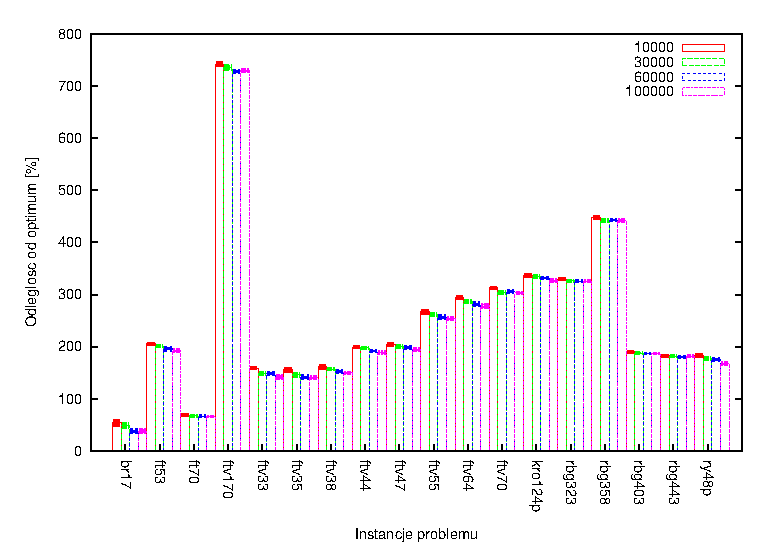
\includegraphics[width=0.9\textwidth]{wykresy/random1}
\end{center}
\caption{Wyniki odległości od optimum dla algorytmu losowego.}
\label{random1}
\end{figure}

\begin{figure}
\begin{center}
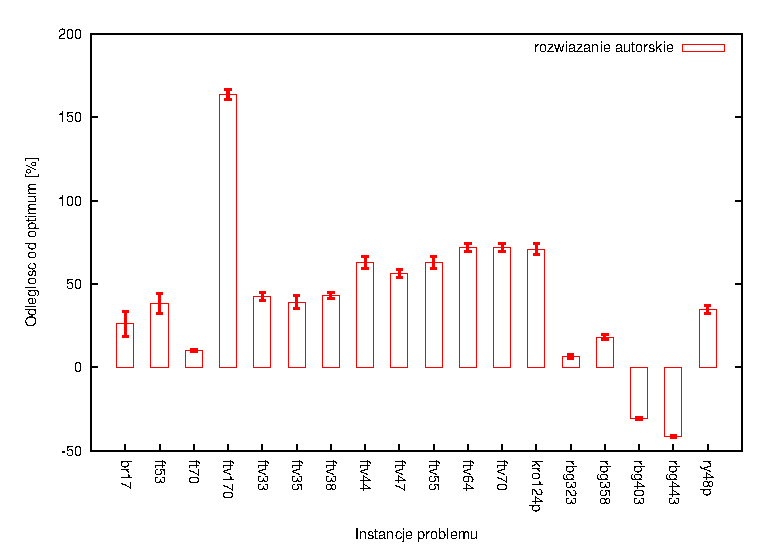
\includegraphics[width=0.9\textwidth]{wykresy/greedy_1}
\end{center}
\caption{Wyniki odległości od optimum dla algorytmu $Greedy$.}
\label{greedy_1}
\end{figure}

\begin{figure}
\begin{center}
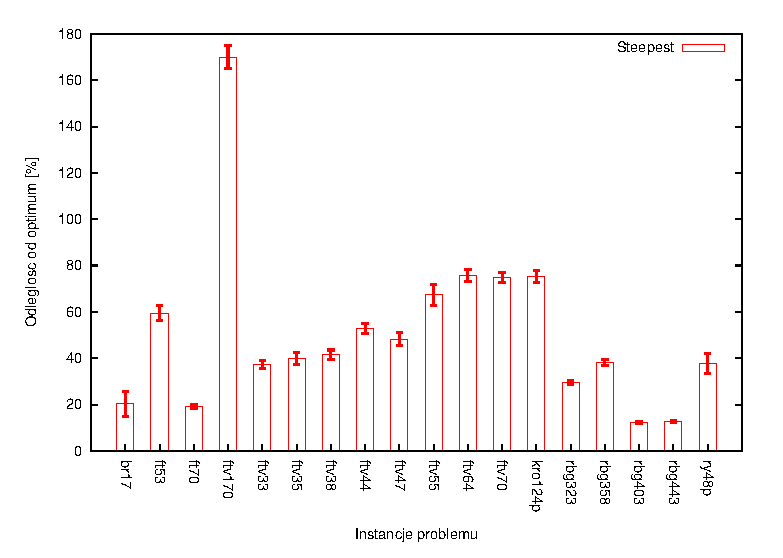
\includegraphics[width=0.9\textwidth]{wykresy/steepest1}
\end{center}
\caption{Wyniki odległości od optimum dla algorytmu $Steepest$.}
\label{steepest1}
\end{figure}

\begin{figure}
\begin{center}
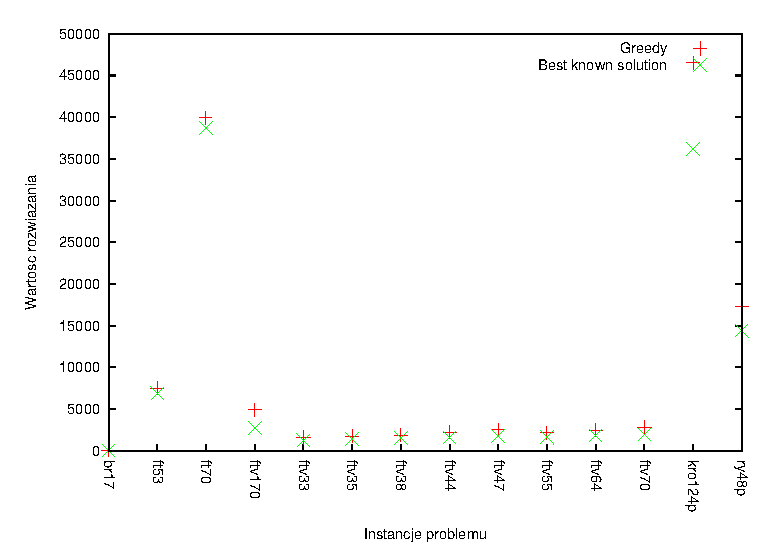
\includegraphics[width=0.9\textwidth]{wykresy/greedy2_1}
\end{center}
\caption{Wyniki odległości od optimum dla algorytmu autorskiego.}
\label{greedy2_1}
\end{figure}

\begin{figure}
\begin{center}
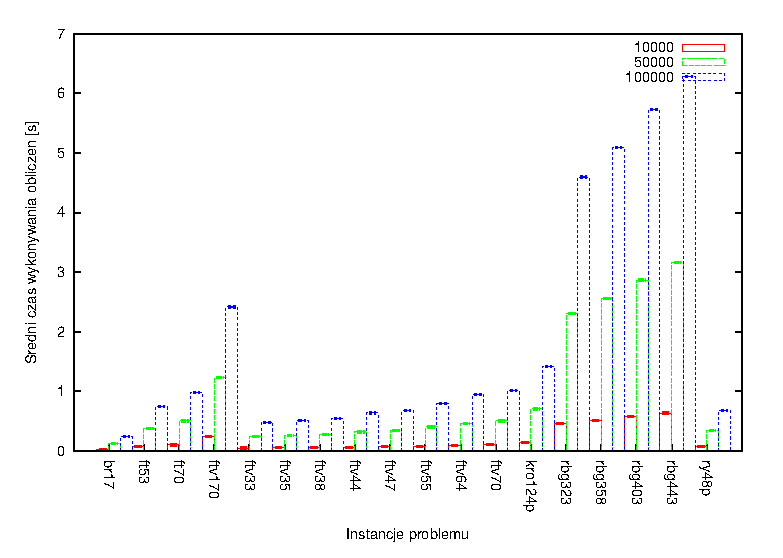
\includegraphics[width=0.9\textwidth]{wykresy/random2}
\end{center}
\caption{Wyniki czasu obliczeń dla algorytmu losowego, w zależności
od liczby losowań.}
\label{random2}
\end{figure}


\begin{figure}
\begin{center}
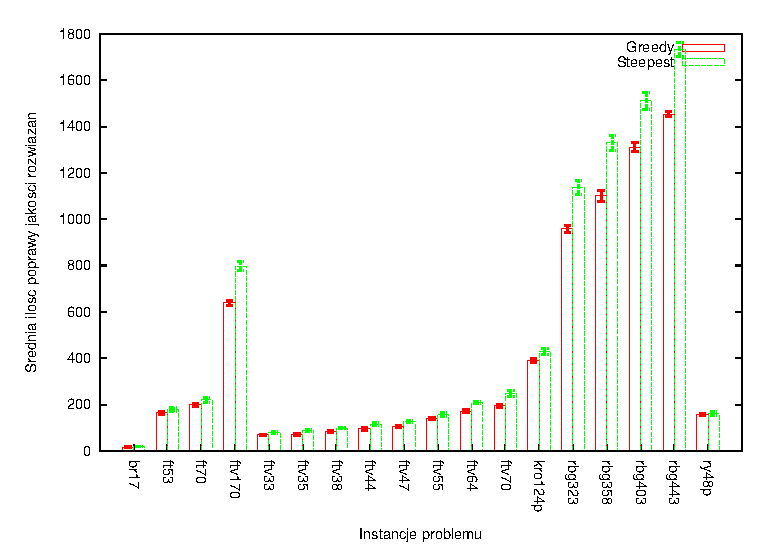
\includegraphics[width=0.9\textwidth]{wykresy/steepest_greedy_better_solutions}
\end{center}
\caption{Liczba popraw wartości rozwiązania podczas przebiegu algorytmu.}
\label{steepest_greedy_better_solutions}
\end{figure}

\begin{figure}
\begin{center}
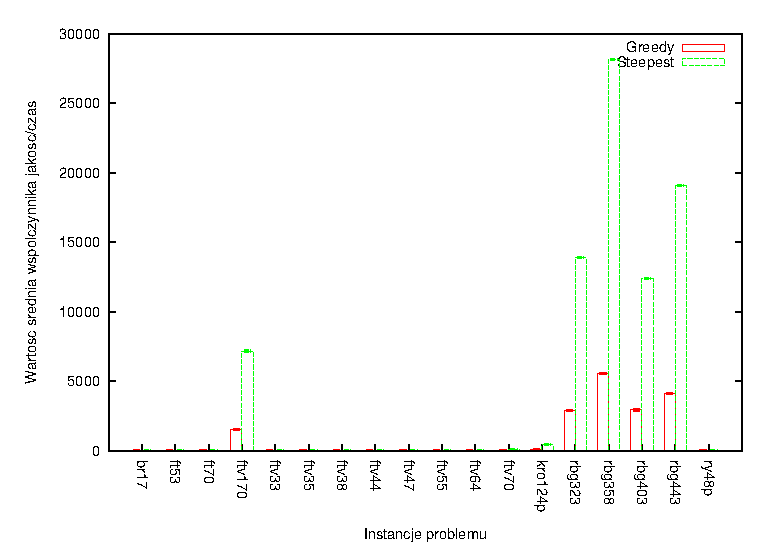
\includegraphics[width=0.9\textwidth]{wykresy/steepest_greedy_czas}
\end{center}
\caption{Czas przetwarzania dla algorytmów $Greedy$ oraz $Steepest$.}
\label{steepest_greedy_czas}
\end{figure}


\begin{figure}
\begin{center}
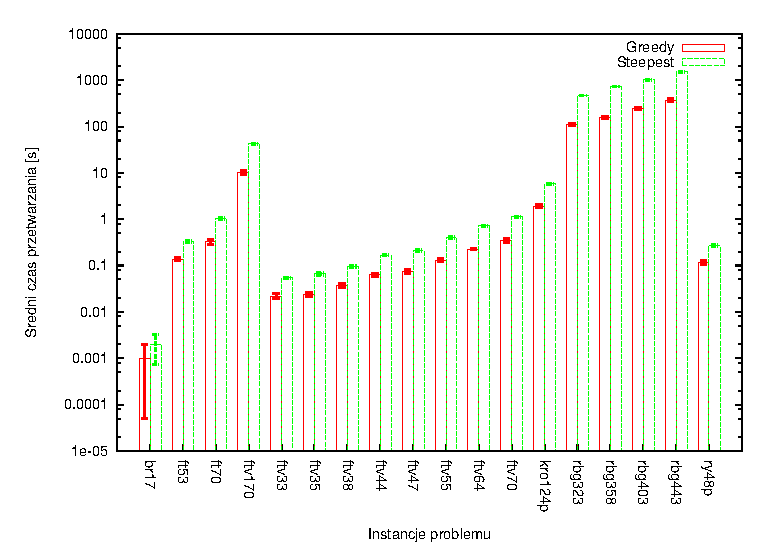
\includegraphics[width=0.9\textwidth]{wykresy/steepest_greedy_czas_log}
\end{center}
\caption{Czas przetwarzania dla algorytmów $Greedy$ oraz $Steepest$ naniesiony
na skali logarytmicznej}
\label{steepest_greedy_czas_log}
\end{figure}

\begin{figure}
\begin{center}
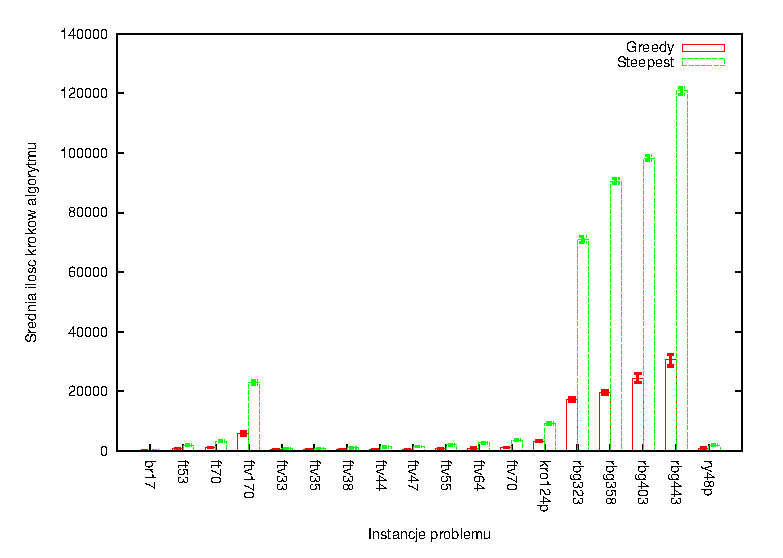
\includegraphics[width=0.9\textwidth]{wykresy/steepest_greedy_steps}
\end{center}
\caption{Ilość kroków wykonanych przez algorytm $Greedy$ oraz $Steepest$.}
\label{steepest_greedy_steps}
\end{figure}

\begin{figure}
\begin{center}
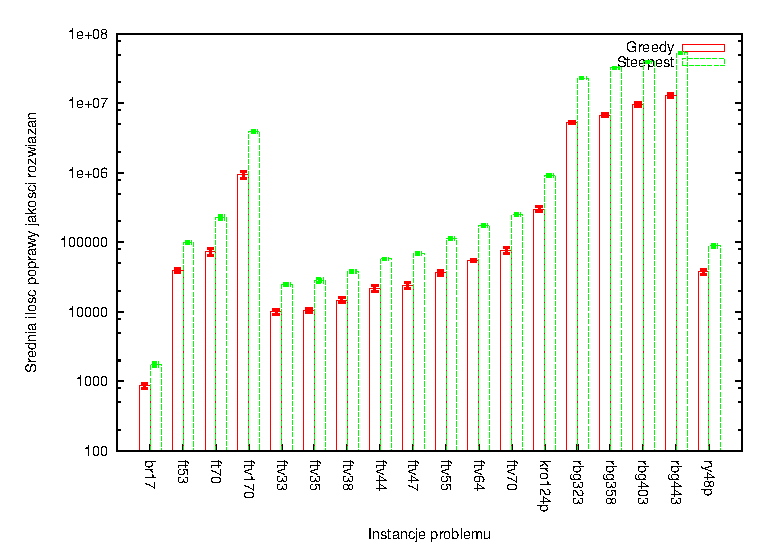
\includegraphics[width=0.9\textwidth]{wykresy/steepest_greedy_visits}
\end{center}
\caption{Ilość odwiedzonych przez algorytmy $Greedy$ oraz $Steepest$
rozwiązań.}
\label{steepest_greedy_visits}
\end{figure}

\begin{figure}
\begin{center}
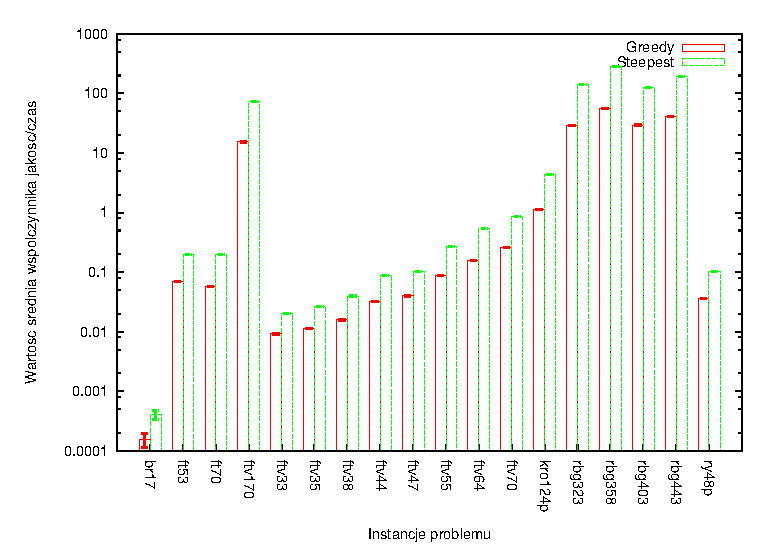
\includegraphics[width=0.9\textwidth]{wykresy/steepest_greedy_jc}
\end{center}
\caption{Miara $jakosc/czas$ dla algorytmów $Greedy$ oraz $Steepest$.}
\label{steepest_greedy_jc}
\end{figure}

\subsection{Jakość rozwiązań}

Po wykonaniu eksperymentów obliczeniowych można dokonać analizy jakości
rozwiązań otrzymanych przez poszczególne algorytmy. Dzięki posiadanym
wartościom miary długości scieżek optymalnych dostępnych na
stronie internetowej $TSPLIB$ możliwe jest określenie dokładności
rozwiązań przybliżonych zwracanych przez algorymty heurystyczne. Patrząc
na otrzymane wyniki można z łatwością stwierdzić, że zaprezentowane
heurystyki zwracają dość dobre wyniki. Wyjątkiem jest algorytm
losowy, dla którego jakość rozwiązań bardzo odbiega od oczekiwanych
rezultatów.

\subsection{Odległość od optimum}

Miarą dokładności rozwiązań jest odległość od optimum
która wyliczana jest jako proporcja wielkości otrzymanej
do wartości optymalnej. Dokładniej rzecz biorąc, jakość rozwiązania
może zostać zapisana w postaci wzoru zamieszczonego poniżej.


$$
\eta =
\left (\frac{f_{obliczone}}{f_{optymalne}} - 1\right )\cdot 100 \%
$$

Na wykresach zamieszczonych poniżej przedstawione są wyniki dokładności
uzyskanych rezultatów dla poszczególnych algorytmów. Oczywiste wydaje się,
że im mniejsza wartość odległości od optimum, tym jakość rozwiążania
jest większa.



\subsection{Czas działania}

W czasie wykonywania eksperymentu obliczeniowego okazało się, że
rozwiązanie autorskie pozwala na znalezienie rozwiązania w bardzo
krótkim czasie, dlatego w niniejszym raporcie czas wykonania
został pominięty. Jest on niewspółmiernie niski w porównaniu do
czasu wykonania pozostałych algorytmów.

Ze względu na bardzo duże zróżnicowanie czasu wykonywania algorytmów
w zależności od rozmiaru instancji, oprócz wyników przedstawionych
na standardowej osi liczbowej, wykonano także wykresy na skali
logarytmicznej, co można zauważyć na rysunku \ref{steepest_greedy_czas}.

\subsection{Jakość/czas}

Ze względu na fakt, bardzo krótkiego czasu wykonania algorytmu
autorskiego, o którym wspomniano w poprzedniej części w czasie analizy
parametru \emph{jakość/czas} nie uwzględniano tego algorytmu.

Do analizy pozostałych przypadków wykorzystano wartości zdefiniowane
w postaci poniższego wzoru, charakteryzującego stosunek \emph{jakość/czas}.

$$
	\lambda = t \cdot \eta
$$

gdzie $\eta$ - jakość rozwiązania; $t$ - czas działania algorytmu.

Nietrudno zauważyć, że rozumienie powyższego parametru jest niezgodne
z intuicyjnym podejściem. Paramter jakość/czas wydawałoby się powinien
przyjmować wysokie wartości w przypadku dobrej jakości rozwiązań. W
przedstawionym przypadku jest jednak inaczej, a więc im mniejsza
wartość tym lepsze okazuje się rozwiązanie. Wyniki
dla rezultatów otrzymanych w przypadku algorytmu $Steepest$ oraz
$Greedy$ zostały zaprezentowane na rysunku nr \ref{steepest_greedy_jc}.

\subsection{Średnia ilość kroków algorytmów}

Kolejną wartością, na którą zwrócono uwagę w czasie eksperymentu
obliczeniowego jest ilość kroków, które zostały wykonane zgodnie
z działaniem algorytmu. Dla algorytmu autorskiego oraz losowego
nie istnieje potrzeba wprowadzania takiej wartości, gdyż ilość
kroków we wspomnianych algorytmach jest znana na początku działania
algorytmu. W przypadku rozwiązania autorskiego ilość krotków jest
równa ilości węzłów w strukturze, natomiast w przypadku algorytmu
losowego jest ustalana przez użytkownika w momencie uruchomienia.


\section{Wnioski}

% Złożność algorytmów
\subsection{Złożoność obliczeniowa prostego algorytmu heurystycznego}

Zgodnie z załączonymi wynikami można zauważyć bardzo którki czas działania prostej
heurystki zaproponowanej przez autorów. Jest to spowodowane kwadratową złożonością 
czasową $ O(n^{2}) $, ponieważ musimy $ n $ razy przejrzeć $ n $ punktów, aby znaleźć
nalbliższy. Otrzymujemy dzięki temu bardzo sybki algorytm. Jego wadą jest 
możliwość otrzymania wyniku bardzo oddalonego od optimum. Dzieje się tak dlatego, 
że przy końcowych obliczeniach nie mamy już dużego wyboru następnych odwiedzanych 
punktów, więc ostatnie ścieżki do wyboru mogę być bardzo długie. Wynik działania 
tego algorytmu mógłby być podstawą do uruchomienia algorymtów Steepest lub Greedy, 
które sprawdziłyby, czy w sąsiedztwie nie leżą lepsze rozwiązania. Znacznie skróciło
by to ich czas działania, poprzez start w miejscu, które jest blisko optimium.
Jest jednak możliwość, że punkt początkowy leżałby w pobliżu jakiegoś optimum 
lokalnego, i zawsze zwracany były ten sam wynik, uniemożliwiając odkrycie innych 
optimów i dzięki temu polepszenie wyniku.

\subsection{Odległość od optimum}

Przedstawione wyniki prezentują, że odległość od optimum dla wykonanych obliczeń 
są bardzo zróżnicowane. Najbardziej stalinie prezentuje się algorytm autorski 
dając średnio 20\% nadłożenie trasy. Algorytmy Steepest i Greedy lepiej działają dla 
większych instancji, przy małych natomiast znajdowane rozwiązania są dalekie od optimum
nawet ponad 2-krotnie.

Najbardziej zmienny jest algorytm losowy. Dane uzyskane za jego pomocą dla małych instancji
potrafią być bliskie optimum, a dla dużych instancji potrafiż byc bardzo odległe. Rozwiązanie
tego specyficznego zachowania zostało wytłumaczone poniżej.

\subsection{Uzyskane wyniki}

Zgodnie z uzyskanymi obliczeniami najlepszy algorytmem okazał się prosty algorytm 
heurystyczny. Uyzkuje on, w niektórych przypadkach, wyniki lepsze o ponad 50\% od
drugiego w zestawieniu algorytmu Greedy. Kolejnym algorytmem jest Steepest z wynikami 
nieznacznie gorszymi od algorytmu Greedy. Ostatni w zestawieniu znalazł się algorytm 
losowy.

\subsubsection{Prosty algorytm heurystyczny}

Sukces algorytmu autorskiego opiera się w dużej części na podejściu do problemu. 
Programowanie dynamiczne wybiera w daej chwili najbardziej optymalne rozwiązanie, 
dzięki czemu osiąga w ogólności bardzo dobre wyniki. Istnieją jednak sytuacje, gdy 
rozwiązania zaproponowane przez prosty algorytm heurystyczny może być ponad 2 razy 
gorsze od pozostałych algorytmów. Dzieje się tak w przypadku, gdy ostatnia wybrana 
trasa jest bardzo długa. Dlatego po otrzymaniu rozwiązania należałoby przejrzeć 
sąsiedztwo w poszukiawaniu rozwiązania lepszego umożliwiając, w niektórych przypadkach
usinięci najdłużeszej trasy.

\subsubsection{Algorytm losowy}

Słaby wynik algorytmu wiąże się z jego niedeterminizmem, jak i brakiem wykorzystania 
już osiągniętych informacji. Jest to jedyny algorytm, dla którego nie można określić 
złożoności, gdyż będzie on działał tak długo, aż jego praca zostanie przerwana. Losując 
rozwiązania na bardzo dużych danych wejściowych ciężko osiąnąć jest wynik nawet zbliżony 
do optimum. 

W przypadku małych instancji algorytm ten zwracał wyniki porównywalne z 
pozostałymi algorytmami w o wiele krótszym czasie (nie licząc czasu działania algorytmu
autorskiego). Dla $ n = 10 $ ilość permutacji wynosi:

$$ n! = 10! = 3~628~800 $$

co przy przykładowych 200~000 powtórzeń daje szansę w trafienie w rozwiązanie optymalne:

$$ \frac{200~000}{10!} * 100\% = 5,51\%  $$

Natomiast jeśli podniesiemy $ n = 50 $ otrzymujemy wyniki:

$$ n! = 50! = 3,04 * 10^{64} $$
$$ \frac{200~000}{50!} * 100\% = 6,58 * 10^{-58}\%  $$

A przy $ n = 400 $, czyli górnej granicy obliczeń:

$$ n! = 400! = 6,40 * 10^{870} $$
$$ \frac{200~000}{400!} * 100\% = 3,13 * 10^{-864}\%  $$

Jak więc widać dla dużych $ n $ szanse trafienia w rozwiązanie optymalne są równe $ 0 $.

Algorytm ten nie wykorzystuje różwnież informacji o już znalezionych rozwiązaniach 
w przypadku generowania nowego, dzięki czemu wygenerowane rozwiązania nie przybliżają
go do optimum.

\subsubsection{Algorytm Greedy i Steepest}

Wyniki uzyskane przez algorytm Greedy są lepsze niż uzyskane przez algorytm Steepest. 
Jest to spowodowane przechodzeniem do najlepszego rozwiązania przez algorytm Steepest. 
Dzięki temu wybiera on najczęściej ścieżkę do najbliższego optimum lokalnego. Algorytm
Greedy natomiast wybiera pierwsze znalezione rozwiązanie, które jest lepsze od dotychczas 
znalezionego. dzięki temu nie zbliża się gwałtownie do żadnego z optimów lokalnych, lecz 
raczej przeszukuje obszar tak długo, aż znajdzie ślepy zaułek.


\subsection{Czas działania}

\it
W zestawieniu nie został ujęty prosty algorytm heurystyczny z poowdu zbyt krótkich czasów 
działania, dla 400 elementów nie został zmierzony (obliczenia pokazywały 0,00), podczas 
gdy najwolniejszy algorytm Steepest wymagał ponad 7 min.
\rm

\subsubsection{Algorytm Greedy}

Czas działania tego algorytmu dla większych instancji jest lepszy o ok. 50 - 70 \% w porównaniu 
do algorytmu Steepest. Pomimo, że potrzebuje on więcej iteracji, przejście do następnego kroku 
zajmuje mniej czasu, gdyż następuje od razu po znalezieniu lepszego rozwiązania. Jego złożoność 
wynosi następująco:

\subsubsection{Algorytm Steepest}

Algorytm ten jest ok. 2 razy gorszy od algorytmu Greedy.Wynika to głównie z fakty, że przegląda on
wszystkie rozwiązania zanim podejmie decyzję o następnym kroku. 

\subsubsection{Algorytm losowy}

Algorytm ten działa niederministycznie, dlatego potrafi osiągnąć szybsze czasy działania dla 
większych instancji. 

\subsection{Ilość iteracji}

Porównując ilość iteracji algorytmów Greedy i Steepest można zauważyć, że algorytm 
Steepest wykonyje ok. 4 razy mniej kroków od algorytmu Greedy. Jest to spowodowane 
dokładnym przeglądaniem przestrzeni sąsiedztwa i wybierania najleprzego rozwiązania.


\section{Napotkane trudności}

\subsection{Błędy implementacji}

W czasie implementacji rozwiązania nie obyło się bez problemów. Bardzo
dużo kłopotów przyspożyły trudne do zlokalizowania bugi. W lokalizacji
pomogło narzędzie gdb, dzieki któremu można było dokonać krok po kroku
fragmenty programu, co do których było podejrzenie że działają niepoprawnie.
Dodatkowo, pomocna okazała się także analiza napisanego wcześniej kodu,
a także inspekcje kodu przeprowadzone w sposób kontroli krzyżowej
przez twórców rozwiązania.

\subsection{Format plików TSP}

Spore trudności podczas pracy były również związane z obsługą plików 
zawierających przykładowe instancjie problemu TSP, pobrane ze strony
internetowej \url{http://comopt.ifi.uni-heidelberg.de/software/TSPLIB95/}.
Nie można było znaleźć biblioteki umożliwiającej sprawne przetwarzanie
plików wejściowych pobranych ze wskazanego źródła. Konieczna okazała
się implementacja własnego modułu pozwalającego zaczytać dane.


\section{Wstęp}

% \begin{figure}
% \begin{center}
% \includegraphics[width=0.4\textwidth]{rys_graf.pdf}
% \end{center}
% \caption{Przyk�adowy schemat z graphviz'a. Przerywane strza�ki oznaczaj�, �e wsz�dzie gdzie si� da u�ywamy grafiki wektorowej -- unikamy wstawiania bitmap do dokumentu. W niekt�rych przypadkach u�ycie bitmap jest uzasadnione (w celu szybkiego podgl�du na ekranie lub dla niezwykle skomplikowanych grafik, zawieraj�cych np.~setki tysi�cy obiekt�w).}
% \label{fig-schemat}
% \end{figure}


To jest przykladowy tekst w LaTeX -- pokazuje jak
% \begin{tightlist}
% \item wstawi� schemat stworzony graphviz'em (Rys.~\ref{fig-schemat}),
% \item wstawi� wykres stworzony gnuplotem (Rys.~\ref{fig-1Tdelta} i \ref{fig-3d}),
% \item zacytowa� literatur� sformatowan� przez bibtex~\cite{MiOIB,Goldberg-2002},
% \item odwo�ywa� si� do rysunk�w, cytowa� i cz��ci sprawozdania (np.\ rozdzia�~\ref{sec-eksperymenty}).
% \end{tightlist}


% \begin{figure}
% \begin{center}
% \includegraphics[width=0.8\textwidth]{rys_wykres2d.pdf}
% \end{center}
% \caption{Przyk�adowy wykres z gnuplota, terminal postscript, zamieniony na pdf za pomoc� programu epstopdf z dystrybucji LaTeX'a (czasem eps2pdf). R��nice $\Delta_{dir}$ warto�ci $p_{dir}$ dla k�ta $90^\circ$.}
% \label{fig-1Tdelta}
% \end{figure}

% \begin{figure}
% \begin{center}
% \includegraphics[width=0.9\textwidth]{rys_wykres3d.pdf}
% \end{center}
% \caption{Jeszcze jeden przyk�adowy wykres z gnuplota.}
% \label{fig-3d}
% \end{figure}




\section{Eksperymenty}
\label{sec-eksperymenty}

W tym rozdziale nic nie ma.




%%%%%%%%%%%%%%%% literatura %%%%%%%%%%%%%%%%

% \bibliography{mioib}
% \bibliographystyle{plain}


\end{document}

